% Options for packages loaded elsewhere
\PassOptionsToPackage{unicode}{hyperref}
\PassOptionsToPackage{hyphens}{url}
\PassOptionsToPackage{dvipsnames,svgnames,x11names}{xcolor}
%
\documentclass[
  letterpaper,
  DIV=11,
  numbers=noendperiod]{scrartcl}

\usepackage{amsmath,amssymb}
\usepackage{iftex}
\ifPDFTeX
  \usepackage[T1]{fontenc}
  \usepackage[utf8]{inputenc}
  \usepackage{textcomp} % provide euro and other symbols
\else % if luatex or xetex
  \usepackage{unicode-math}
  \defaultfontfeatures{Scale=MatchLowercase}
  \defaultfontfeatures[\rmfamily]{Ligatures=TeX,Scale=1}
\fi
\usepackage{lmodern}
\ifPDFTeX\else  
    % xetex/luatex font selection
\fi
% Use upquote if available, for straight quotes in verbatim environments
\IfFileExists{upquote.sty}{\usepackage{upquote}}{}
\IfFileExists{microtype.sty}{% use microtype if available
  \usepackage[]{microtype}
  \UseMicrotypeSet[protrusion]{basicmath} % disable protrusion for tt fonts
}{}
\makeatletter
\@ifundefined{KOMAClassName}{% if non-KOMA class
  \IfFileExists{parskip.sty}{%
    \usepackage{parskip}
  }{% else
    \setlength{\parindent}{0pt}
    \setlength{\parskip}{6pt plus 2pt minus 1pt}}
}{% if KOMA class
  \KOMAoptions{parskip=half}}
\makeatother
\usepackage{xcolor}
\setlength{\emergencystretch}{3em} % prevent overfull lines
\setcounter{secnumdepth}{-\maxdimen} % remove section numbering
% Make \paragraph and \subparagraph free-standing
\ifx\paragraph\undefined\else
  \let\oldparagraph\paragraph
  \renewcommand{\paragraph}[1]{\oldparagraph{#1}\mbox{}}
\fi
\ifx\subparagraph\undefined\else
  \let\oldsubparagraph\subparagraph
  \renewcommand{\subparagraph}[1]{\oldsubparagraph{#1}\mbox{}}
\fi

\usepackage{color}
\usepackage{fancyvrb}
\newcommand{\VerbBar}{|}
\newcommand{\VERB}{\Verb[commandchars=\\\{\}]}
\DefineVerbatimEnvironment{Highlighting}{Verbatim}{commandchars=\\\{\}}
% Add ',fontsize=\small' for more characters per line
\usepackage{framed}
\definecolor{shadecolor}{RGB}{241,243,245}
\newenvironment{Shaded}{\begin{snugshade}}{\end{snugshade}}
\newcommand{\AlertTok}[1]{\textcolor[rgb]{0.68,0.00,0.00}{#1}}
\newcommand{\AnnotationTok}[1]{\textcolor[rgb]{0.37,0.37,0.37}{#1}}
\newcommand{\AttributeTok}[1]{\textcolor[rgb]{0.40,0.45,0.13}{#1}}
\newcommand{\BaseNTok}[1]{\textcolor[rgb]{0.68,0.00,0.00}{#1}}
\newcommand{\BuiltInTok}[1]{\textcolor[rgb]{0.00,0.23,0.31}{#1}}
\newcommand{\CharTok}[1]{\textcolor[rgb]{0.13,0.47,0.30}{#1}}
\newcommand{\CommentTok}[1]{\textcolor[rgb]{0.37,0.37,0.37}{#1}}
\newcommand{\CommentVarTok}[1]{\textcolor[rgb]{0.37,0.37,0.37}{\textit{#1}}}
\newcommand{\ConstantTok}[1]{\textcolor[rgb]{0.56,0.35,0.01}{#1}}
\newcommand{\ControlFlowTok}[1]{\textcolor[rgb]{0.00,0.23,0.31}{#1}}
\newcommand{\DataTypeTok}[1]{\textcolor[rgb]{0.68,0.00,0.00}{#1}}
\newcommand{\DecValTok}[1]{\textcolor[rgb]{0.68,0.00,0.00}{#1}}
\newcommand{\DocumentationTok}[1]{\textcolor[rgb]{0.37,0.37,0.37}{\textit{#1}}}
\newcommand{\ErrorTok}[1]{\textcolor[rgb]{0.68,0.00,0.00}{#1}}
\newcommand{\ExtensionTok}[1]{\textcolor[rgb]{0.00,0.23,0.31}{#1}}
\newcommand{\FloatTok}[1]{\textcolor[rgb]{0.68,0.00,0.00}{#1}}
\newcommand{\FunctionTok}[1]{\textcolor[rgb]{0.28,0.35,0.67}{#1}}
\newcommand{\ImportTok}[1]{\textcolor[rgb]{0.00,0.46,0.62}{#1}}
\newcommand{\InformationTok}[1]{\textcolor[rgb]{0.37,0.37,0.37}{#1}}
\newcommand{\KeywordTok}[1]{\textcolor[rgb]{0.00,0.23,0.31}{#1}}
\newcommand{\NormalTok}[1]{\textcolor[rgb]{0.00,0.23,0.31}{#1}}
\newcommand{\OperatorTok}[1]{\textcolor[rgb]{0.37,0.37,0.37}{#1}}
\newcommand{\OtherTok}[1]{\textcolor[rgb]{0.00,0.23,0.31}{#1}}
\newcommand{\PreprocessorTok}[1]{\textcolor[rgb]{0.68,0.00,0.00}{#1}}
\newcommand{\RegionMarkerTok}[1]{\textcolor[rgb]{0.00,0.23,0.31}{#1}}
\newcommand{\SpecialCharTok}[1]{\textcolor[rgb]{0.37,0.37,0.37}{#1}}
\newcommand{\SpecialStringTok}[1]{\textcolor[rgb]{0.13,0.47,0.30}{#1}}
\newcommand{\StringTok}[1]{\textcolor[rgb]{0.13,0.47,0.30}{#1}}
\newcommand{\VariableTok}[1]{\textcolor[rgb]{0.07,0.07,0.07}{#1}}
\newcommand{\VerbatimStringTok}[1]{\textcolor[rgb]{0.13,0.47,0.30}{#1}}
\newcommand{\WarningTok}[1]{\textcolor[rgb]{0.37,0.37,0.37}{\textit{#1}}}

\providecommand{\tightlist}{%
  \setlength{\itemsep}{0pt}\setlength{\parskip}{0pt}}\usepackage{longtable,booktabs,array}
\usepackage{calc} % for calculating minipage widths
% Correct order of tables after \paragraph or \subparagraph
\usepackage{etoolbox}
\makeatletter
\patchcmd\longtable{\par}{\if@noskipsec\mbox{}\fi\par}{}{}
\makeatother
% Allow footnotes in longtable head/foot
\IfFileExists{footnotehyper.sty}{\usepackage{footnotehyper}}{\usepackage{footnote}}
\makesavenoteenv{longtable}
\usepackage{graphicx}
\makeatletter
\def\maxwidth{\ifdim\Gin@nat@width>\linewidth\linewidth\else\Gin@nat@width\fi}
\def\maxheight{\ifdim\Gin@nat@height>\textheight\textheight\else\Gin@nat@height\fi}
\makeatother
% Scale images if necessary, so that they will not overflow the page
% margins by default, and it is still possible to overwrite the defaults
% using explicit options in \includegraphics[width, height, ...]{}
\setkeys{Gin}{width=\maxwidth,height=\maxheight,keepaspectratio}
% Set default figure placement to htbp
\makeatletter
\def\fps@figure{htbp}
\makeatother

\KOMAoption{captions}{tableheading}
\makeatletter
\makeatother
\makeatletter
\makeatother
\makeatletter
\@ifpackageloaded{caption}{}{\usepackage{caption}}
\AtBeginDocument{%
\ifdefined\contentsname
  \renewcommand*\contentsname{Table of contents}
\else
  \newcommand\contentsname{Table of contents}
\fi
\ifdefined\listfigurename
  \renewcommand*\listfigurename{List of Figures}
\else
  \newcommand\listfigurename{List of Figures}
\fi
\ifdefined\listtablename
  \renewcommand*\listtablename{List of Tables}
\else
  \newcommand\listtablename{List of Tables}
\fi
\ifdefined\figurename
  \renewcommand*\figurename{Figure}
\else
  \newcommand\figurename{Figure}
\fi
\ifdefined\tablename
  \renewcommand*\tablename{Table}
\else
  \newcommand\tablename{Table}
\fi
}
\@ifpackageloaded{float}{}{\usepackage{float}}
\floatstyle{ruled}
\@ifundefined{c@chapter}{\newfloat{codelisting}{h}{lop}}{\newfloat{codelisting}{h}{lop}[chapter]}
\floatname{codelisting}{Listing}
\newcommand*\listoflistings{\listof{codelisting}{List of Listings}}
\makeatother
\makeatletter
\@ifpackageloaded{caption}{}{\usepackage{caption}}
\@ifpackageloaded{subcaption}{}{\usepackage{subcaption}}
\makeatother
\makeatletter
\@ifpackageloaded{tcolorbox}{}{\usepackage[skins,breakable]{tcolorbox}}
\makeatother
\makeatletter
\@ifundefined{shadecolor}{\definecolor{shadecolor}{rgb}{.97, .97, .97}}
\makeatother
\makeatletter
\makeatother
\makeatletter
\makeatother
\ifLuaTeX
  \usepackage{selnolig}  % disable illegal ligatures
\fi
\IfFileExists{bookmark.sty}{\usepackage{bookmark}}{\usepackage{hyperref}}
\IfFileExists{xurl.sty}{\usepackage{xurl}}{} % add URL line breaks if available
\urlstyle{same} % disable monospaced font for URLs
\hypersetup{
  pdftitle={ANOVA},
  pdfauthor={Nicolas Jadan},
  colorlinks=true,
  linkcolor={blue},
  filecolor={Maroon},
  citecolor={Blue},
  urlcolor={Blue},
  pdfcreator={LaTeX via pandoc}}

\title{ANOVA}
\author{Nicolas Jadan}
\date{}

\begin{document}
\maketitle
\ifdefined\Shaded\renewenvironment{Shaded}{\begin{tcolorbox}[boxrule=0pt, sharp corners, interior hidden, frame hidden, enhanced, borderline west={3pt}{0pt}{shadecolor}, breakable]}{\end{tcolorbox}}\fi

\hypertarget{visualice-sus-datos-y-calcule-anova-unidireccional-en-r}{%
\section{Visualice sus datos y calcule ANOVA unidireccional en
R}\label{visualice-sus-datos-y-calcule-anova-unidireccional-en-r}}

\hypertarget{importar-los-datos-a-r}{%
\subsection{Importar los datos a R}\label{importar-los-datos-a-r}}

\begin{Shaded}
\begin{Highlighting}[]
\CommentTok{\# Or, if .csv file, use this}
\NormalTok{my\_data }\OtherTok{\textless{}{-}} \FunctionTok{read.csv}\NormalTok{(}\StringTok{"cancer.csv"}\NormalTok{)}
\end{Highlighting}
\end{Shaded}

\hypertarget{comprueba-tus-datos}{%
\subsection{Comprueba tus datos}\label{comprueba-tus-datos}}

Para tener una idea de cómo se ven los datos, usamos la función
\textbf{sample\_n}(){[}en el paquete \textbf{dplyr}{]}. La función
\textbf{sample\_n}() selecciona aleatoriamente algunas de las
observaciones en el marco de datos para imprimir:

\begin{Shaded}
\begin{Highlighting}[]
\CommentTok{\# Show a random sample}
\FunctionTok{set.seed}\NormalTok{(}\DecValTok{1234}\NormalTok{)}
\NormalTok{dplyr}\SpecialCharTok{::}\FunctionTok{sample\_n}\NormalTok{(my\_data, }\DecValTok{10}\NormalTok{)}
\end{Highlighting}
\end{Shaded}

\begin{verbatim}
   group weight
1      M 16.240
2      M 13.610
3      B 11.800
4      B  9.787
5      B 12.180
6      B 12.670
7      M 20.180
8      B 10.710
9      B 11.040
10     B 11.410
\end{verbatim}

\begin{itemize}
\tightlist
\item
  Calcular estadísticas de resumen por grupos: recuento, media, sd:
\end{itemize}

\begin{Shaded}
\begin{Highlighting}[]
\CommentTok{\# Show the levels}
\FunctionTok{levels}\NormalTok{(my\_data}\SpecialCharTok{$}\NormalTok{group)}
\end{Highlighting}
\end{Shaded}

\begin{verbatim}
NULL
\end{verbatim}

\begin{Shaded}
\begin{Highlighting}[]
\NormalTok{my\_data}\SpecialCharTok{$}\NormalTok{group }\OtherTok{\textless{}{-}} \FunctionTok{ordered}\NormalTok{(my\_data}\SpecialCharTok{$}\NormalTok{group,}
                         \AttributeTok{levels =} \FunctionTok{c}\NormalTok{(}\StringTok{"B"}\NormalTok{, }\StringTok{"M"}\NormalTok{))}
\FunctionTok{library}\NormalTok{(dplyr)}
\end{Highlighting}
\end{Shaded}

\begin{verbatim}

Attaching package: 'dplyr'
\end{verbatim}

\begin{verbatim}
The following objects are masked from 'package:stats':

    filter, lag
\end{verbatim}

\begin{verbatim}
The following objects are masked from 'package:base':

    intersect, setdiff, setequal, union
\end{verbatim}

\begin{Shaded}
\begin{Highlighting}[]
\FunctionTok{group\_by}\NormalTok{(my\_data, group) }\SpecialCharTok{\%\textgreater{}\%}
  \FunctionTok{summarise}\NormalTok{(}
    \AttributeTok{count =} \FunctionTok{n}\NormalTok{(),}
    \AttributeTok{mean =} \FunctionTok{mean}\NormalTok{(weight, }\AttributeTok{na.rm =} \ConstantTok{TRUE}\NormalTok{),}
    \AttributeTok{sd =} \FunctionTok{sd}\NormalTok{(weight, }\AttributeTok{na.rm =} \ConstantTok{TRUE}\NormalTok{)}
\NormalTok{  )}
\end{Highlighting}
\end{Shaded}

\begin{verbatim}
# A tibble: 2 x 4
  group count  mean    sd
  <ord> <int> <dbl> <dbl>
1 B       357  12.1  1.78
2 M       212  17.5  3.20
\end{verbatim}

\hypertarget{visualiza-tus-datos}{%
\subsection{Visualiza tus datos}\label{visualiza-tus-datos}}

\begin{itemize}
\item
  Para usar gráficos base de R, lea esto:
  \href{http://www.sthda.com/english/wiki/r-base-graphs}{Gráficos de
  base de R}. Aquí, usaremos el
  \href{http://www.sthda.com/english/wiki/ggpubr-r-package-ggplot2-based-publication-ready-plots}{paquete
  \textbf{ggpubr} R} para una fácil visualización de datos basada en
  ggplot2.
\item
  Visualiza tus datos con ggpubr:
\end{itemize}

\begin{Shaded}
\begin{Highlighting}[]
\CommentTok{\# Box plots}
\CommentTok{\# ++++++++++++++++++++}
\CommentTok{\# Plot weight by group and color by group}
\FunctionTok{library}\NormalTok{(}\StringTok{"ggpubr"}\NormalTok{)}
\end{Highlighting}
\end{Shaded}

\begin{verbatim}
Warning: package 'ggpubr' was built under R version 4.3.1
\end{verbatim}

\begin{verbatim}
Loading required package: ggplot2
\end{verbatim}

\begin{Shaded}
\begin{Highlighting}[]
\FunctionTok{ggboxplot}\NormalTok{(my\_data, }\AttributeTok{x =} \StringTok{"group"}\NormalTok{, }\AttributeTok{y =} \StringTok{"weight"}\NormalTok{, }
          \AttributeTok{color =} \StringTok{"group"}\NormalTok{, }\AttributeTok{palette =} \FunctionTok{c}\NormalTok{(}\StringTok{"\#00AFBB"}\NormalTok{, }\StringTok{"\#E7B800"}\NormalTok{, }\StringTok{"\#FC4E07"}\NormalTok{),}
          \AttributeTok{order =} \FunctionTok{c}\NormalTok{(}\StringTok{"B"}\NormalTok{, }\StringTok{"M"}\NormalTok{),}
          \AttributeTok{ylab =} \StringTok{"Weight"}\NormalTok{, }\AttributeTok{xlab =} \StringTok{"Treatment"}\NormalTok{)}
\end{Highlighting}
\end{Shaded}

\begin{figure}[H]

{\centering 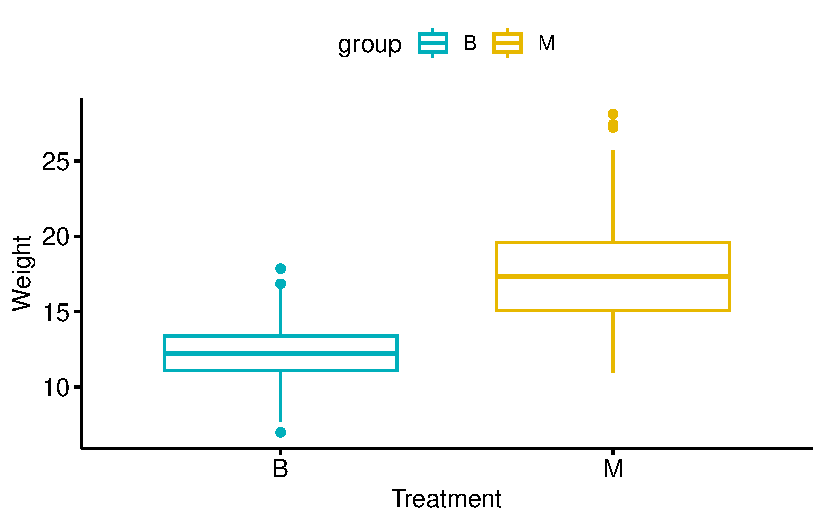
\includegraphics{ANOVA_files/figure-pdf/unnamed-chunk-4-1.pdf}

}

\end{figure}

\begin{Shaded}
\begin{Highlighting}[]
\CommentTok{\# Mean plots}
\CommentTok{\# ++++++++++++++++++++}
\CommentTok{\# Plot weight by group}
\CommentTok{\# Add error bars: mean\_se}
\CommentTok{\# (other values include: mean\_sd, mean\_ci, median\_iqr, ....)}
\FunctionTok{library}\NormalTok{(}\StringTok{"ggpubr"}\NormalTok{)}
\FunctionTok{ggline}\NormalTok{(my\_data, }\AttributeTok{x =} \StringTok{"group"}\NormalTok{, }\AttributeTok{y =} \StringTok{"weight"}\NormalTok{, }
       \AttributeTok{add =} \FunctionTok{c}\NormalTok{(}\StringTok{"mean\_se"}\NormalTok{, }\StringTok{"jitter"}\NormalTok{), }
       \AttributeTok{order =} \FunctionTok{c}\NormalTok{(}\StringTok{"B"}\NormalTok{, }\StringTok{"M"}\NormalTok{),}
       \AttributeTok{ylab =} \StringTok{"Weight"}\NormalTok{, }\AttributeTok{xlab =} \StringTok{"Treatment"}\NormalTok{)}
\end{Highlighting}
\end{Shaded}

\begin{figure}[H]

{\centering 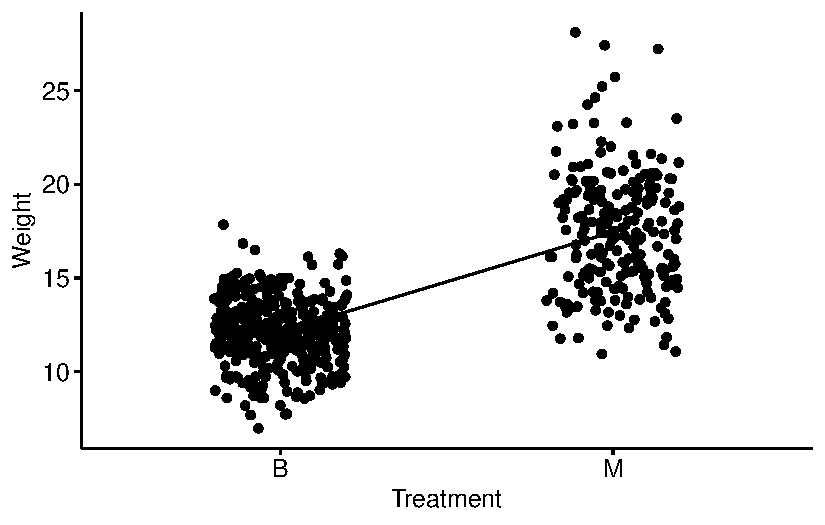
\includegraphics{ANOVA_files/figure-pdf/unnamed-chunk-5-1.pdf}

}

\end{figure}

\begin{Shaded}
\begin{Highlighting}[]
\CommentTok{\# Box plot}
\FunctionTok{boxplot}\NormalTok{(weight }\SpecialCharTok{\textasciitilde{}}\NormalTok{ group, }\AttributeTok{data =}\NormalTok{ my\_data,}
        \AttributeTok{xlab =} \StringTok{"Treatment"}\NormalTok{, }\AttributeTok{ylab =} \StringTok{"Weight"}\NormalTok{,}
        \AttributeTok{frame =} \ConstantTok{FALSE}\NormalTok{, }\AttributeTok{col =} \FunctionTok{c}\NormalTok{(}\StringTok{"\#00AFBB"}\NormalTok{, }\StringTok{"\#E7B800"}\NormalTok{, }\StringTok{"\#FC4E07"}\NormalTok{))}
\end{Highlighting}
\end{Shaded}

\begin{figure}[H]

{\centering 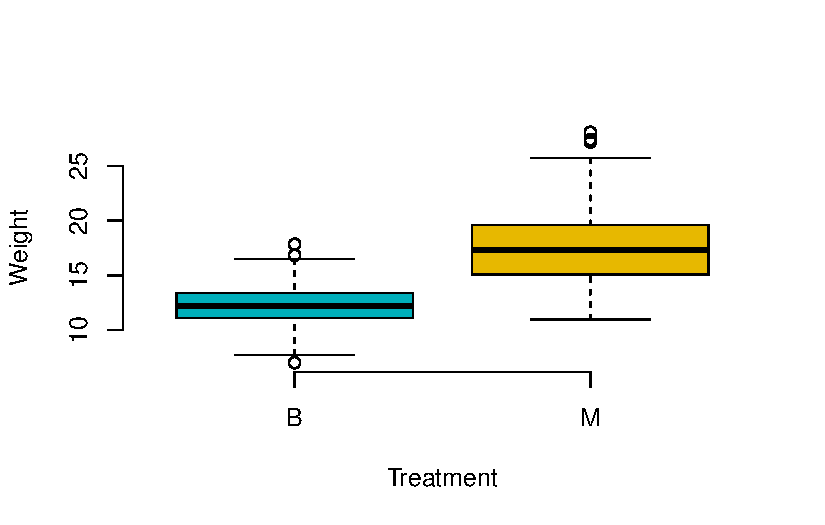
\includegraphics{ANOVA_files/figure-pdf/unnamed-chunk-5-2.pdf}

}

\end{figure}

\begin{Shaded}
\begin{Highlighting}[]
\CommentTok{\# plotmeans}
\FunctionTok{library}\NormalTok{(}\StringTok{"gplots"}\NormalTok{)}
\end{Highlighting}
\end{Shaded}

\begin{verbatim}
Warning: package 'gplots' was built under R version 4.3.1
\end{verbatim}

\begin{verbatim}

Attaching package: 'gplots'
\end{verbatim}

\begin{verbatim}
The following object is masked from 'package:stats':

    lowess
\end{verbatim}

\begin{Shaded}
\begin{Highlighting}[]
\FunctionTok{plotmeans}\NormalTok{(weight }\SpecialCharTok{\textasciitilde{}}\NormalTok{ group, }\AttributeTok{data =}\NormalTok{ my\_data, }\AttributeTok{frame =} \ConstantTok{FALSE}\NormalTok{,}
          \AttributeTok{xlab =} \StringTok{"Treatment"}\NormalTok{, }\AttributeTok{ylab =} \StringTok{"Weight"}\NormalTok{,}
          \AttributeTok{main=}\StringTok{"Mean Plot with 95\% CI"}\NormalTok{) }
\end{Highlighting}
\end{Shaded}

\begin{verbatim}
Warning in arrows(x, li, x, pmax(y - gap, li), col = barcol, lwd = lwd, :
zero-length arrow is of indeterminate angle and so skipped
\end{verbatim}

\begin{verbatim}
Warning in arrows(x, li, x, pmax(y - gap, li), col = barcol, lwd = lwd, :
zero-length arrow is of indeterminate angle and so skipped
\end{verbatim}

\begin{verbatim}
Warning in arrows(x, ui, x, pmin(y + gap, ui), col = barcol, lwd = lwd, :
zero-length arrow is of indeterminate angle and so skipped

Warning in arrows(x, ui, x, pmin(y + gap, ui), col = barcol, lwd = lwd, :
zero-length arrow is of indeterminate angle and so skipped
\end{verbatim}

\begin{verbatim}
Warning in plot.xy(xy.coords(x, y), type = type, ...): "frame" is not a
graphical parameter
\end{verbatim}

\begin{verbatim}
Warning in axis(1, at = 1:length(means), labels = legends, ...): "frame" is not
a graphical parameter
\end{verbatim}

\begin{verbatim}
Warning in plot.xy(xy.coords(x, y), type = type, ...): "frame" is not a
graphical parameter
\end{verbatim}

\begin{figure}[H]

{\centering 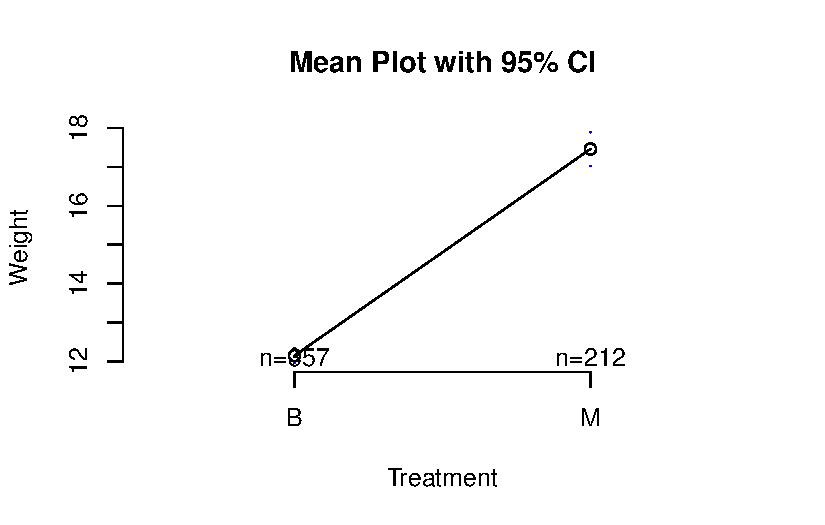
\includegraphics{ANOVA_files/figure-pdf/unnamed-chunk-5-3.pdf}

}

\end{figure}

\hypertarget{calcular-la-prueba-anova-unidireccional}{%
\subsection{Calcular la prueba ANOVA
unidireccional}\label{calcular-la-prueba-anova-unidireccional}}

La función R~\textbf{aov}() se puede utilizar para responder a esta
pregunta. La función~\textbf{summary.aov}() se utiliza para resumir el
modelo de análisis de varianza.

\begin{Shaded}
\begin{Highlighting}[]
\CommentTok{\# Compute the analysis of variance}
\NormalTok{res.aov }\OtherTok{\textless{}{-}} \FunctionTok{aov}\NormalTok{(weight }\SpecialCharTok{\textasciitilde{}}\NormalTok{ group, }\AttributeTok{data =}\NormalTok{ my\_data)}
\CommentTok{\# Summary of the analysis}
\FunctionTok{summary}\NormalTok{(res.aov)}
\end{Highlighting}
\end{Shaded}

\begin{verbatim}
             Df Sum Sq Mean Sq F value Pr(>F)    
group         1   3759    3759     647 <2e-16 ***
Residuals   567   3295       6                   
---
Signif. codes:  0 '***' 0.001 '**' 0.01 '*' 0.05 '.' 0.1 ' ' 1
\end{verbatim}

\hypertarget{interpretar-el-resultado-de-las-pruebas-anova-unidireccionales}{%
\subsection{Interpretar el resultado de las pruebas ANOVA
unidireccionales}\label{interpretar-el-resultado-de-las-pruebas-anova-unidireccionales}}

Como el valor p es menor que el nivel de significancia 0,05, podemos
concluir que existen diferencias significativas entre los grupos
resaltados con ``*'' en el resumen del modelo.

\hypertarget{comparaciuxf3n-muxfaltiple-por-pares-entre-las-medias-de-los-grupos}{%
\subsection{Comparación múltiple por pares entre las medias de los
grupos}\label{comparaciuxf3n-muxfaltiple-por-pares-entre-las-medias-de-los-grupos}}

En la prueba ANOVA unidireccional, un valor p significativo indica que
algunas de las medias grupales son diferentes, pero no sabemos qué pares
de grupos son diferentes.

Es posible realizar múltiples comparaciones por pares, para determinar
si la diferencia media entre pares específicos de grupo es
estadísticamente significativa.

\hypertarget{comparaciones-muxfaltiples-por-pares-de-tukey}{%
\subsubsection{Comparaciones múltiples por pares de
Tukey}\label{comparaciones-muxfaltiples-por-pares-de-tukey}}

Como la prueba ANOVA es significativa, podemos calcular Tukey
\textbf{HSD (Tukey} Honest Significant Differences, función R:
\textbf{TukeyHSD}()) para realizar múltiples comparaciones por pares
entre las medias de los grupos.

La función \textbf{TukeyHD(}) toma el ANOVA instalado como argumento.

\begin{Shaded}
\begin{Highlighting}[]
\FunctionTok{TukeyHSD}\NormalTok{(res.aov)}
\end{Highlighting}
\end{Shaded}

\begin{verbatim}
  Tukey multiple comparisons of means
    95% family-wise confidence level

Fit: aov(formula = weight ~ group, data = my_data)

$group
        diff      lwr      upr p adj
M-B 5.316306 4.905781 5.726832     0
\end{verbatim}

\begin{itemize}
\item
  \textbf{diff}: diferencia entre las medias de los dos grupos
\item
  \textbf{LWR}, \textbf{UPR}: el punto final inferior y superior del
  intervalo de confianza al 95\% (predeterminado)
\item
  \textbf{p adj}: valor p después del ajuste para las comparaciones
  múltiples.

  \hypertarget{comparaciones-muxfaltiples-usando-el-paquete-multcomp}{%
  \subsubsection{Comparaciones múltiples usando el paquete
  multcomp}\label{comparaciones-muxfaltiples-usando-el-paquete-multcomp}}

  Es posible usar la función \textbf{glht}() {[}en el paquete
  \textbf{multcomp}{]} para realizar múltiples procedimientos de
  comparación para un ANOVA. \textbf{GLHT} significa pruebas generales
  de hipótesis lineales. El formato simplificado es el siguiente:
\end{itemize}

\begin{Shaded}
\begin{Highlighting}[]
\CommentTok{\#summary(glht(res.aov, linfct = mcp(group = "Tukey")))}
\end{Highlighting}
\end{Shaded}

\hypertarget{prueba-t-de-pairewise}{%
\subsubsection{Prueba t de Pairewise}\label{prueba-t-de-pairewise}}

La función \textbf{pairewise.t.test}() también se puede utilizar para
calcular comparaciones por pares entre niveles de grupo con correcciones
para pruebas múltiples.

\begin{Shaded}
\begin{Highlighting}[]
\FunctionTok{pairwise.t.test}\NormalTok{(my\_data}\SpecialCharTok{$}\NormalTok{weight, my\_data}\SpecialCharTok{$}\NormalTok{group,}
                 \AttributeTok{p.adjust.method =} \StringTok{"BH"}\NormalTok{)}
\end{Highlighting}
\end{Shaded}

\begin{verbatim}

    Pairwise comparisons using t tests with pooled SD 

data:  my_data$weight and my_data$group 

  B     
M <2e-16

P value adjustment method: BH 
\end{verbatim}

El resultado es una tabla de valores p para las comparaciones por pares.
Aquí, los valores p han sido ajustados por el método de
Benjamini-Hochberg.

\hypertarget{verifique-los-supuestos-de-anova-validez-de-la-prueba}{%
\subsection{Verifique los supuestos de ANOVA: ¿validez de la
prueba?}\label{verifique-los-supuestos-de-anova-validez-de-la-prueba}}

La prueba ANOVA asume que los datos se distribuyen normalmente y la
varianza entre los grupos es homogénea. Podemos comprobarlo con algunas
gráficas diagnósticas.

\hypertarget{comprobar-la-homogeneidad-de-la-hipuxf3tesis-de-varianza}{%
\subsubsection{Comprobar la homogeneidad de la hipótesis de
varianza}\label{comprobar-la-homogeneidad-de-la-hipuxf3tesis-de-varianza}}

La \textbf{gráfica de residuos versus ajustes} se puede utilizar para
verificar la homogeneidad de las varianzas.

En la siguiente gráfica, no hay relaciones evidentes entre los residuos
y los valores ajustados (la media de cada grupo), lo cual es bueno. Por
lo tanto, podemos asumir la homogeneidad de las varianzas.

\begin{Shaded}
\begin{Highlighting}[]
\CommentTok{\# 1. Homogeneity of variances}
\FunctionTok{plot}\NormalTok{(res.aov, }\DecValTok{1}\NormalTok{)}
\end{Highlighting}
\end{Shaded}

\begin{figure}[H]

{\centering 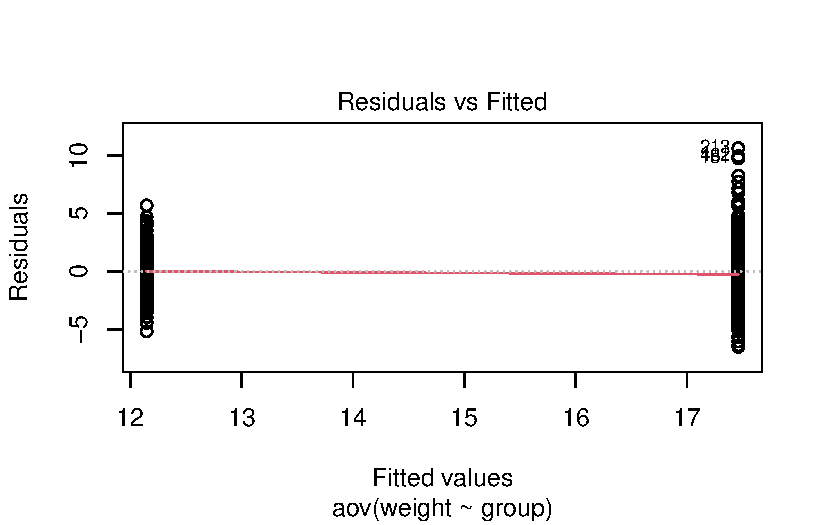
\includegraphics{ANOVA_files/figure-pdf/unnamed-chunk-10-1.pdf}

}

\end{figure}

Recomendamos la \textbf{prueba de Levene}, que es menos sensible a las
desviaciones de la distribución normal. Se utilizará la función
\textbf{leveneTest}() {[}en \textbf{el paquete car}{]}:

\begin{Shaded}
\begin{Highlighting}[]
\FunctionTok{library}\NormalTok{(car)}
\end{Highlighting}
\end{Shaded}

\begin{verbatim}
Loading required package: carData
\end{verbatim}

\begin{verbatim}

Attaching package: 'car'
\end{verbatim}

\begin{verbatim}
The following object is masked from 'package:dplyr':

    recode
\end{verbatim}

\begin{Shaded}
\begin{Highlighting}[]
\FunctionTok{leveneTest}\NormalTok{(weight }\SpecialCharTok{\textasciitilde{}}\NormalTok{ group, }\AttributeTok{data =}\NormalTok{ my\_data)}
\end{Highlighting}
\end{Shaded}

\begin{verbatim}
Levene's Test for Homogeneity of Variance (center = median)
       Df F value    Pr(>F)    
group   1  90.477 < 2.2e-16 ***
      567                      
---
Signif. codes:  0 '***' 0.001 '**' 0.01 '*' 0.05 '.' 0.1 ' ' 1
\end{verbatim}

De la salida anterior podemos ver que el valor p no es menor que el
nivel de significación de 0.05. Esto significa que no hay evidencia que
sugiera que la varianza entre los grupos sea estadísticamente
significativamente diferente. Por lo tanto, podemos asumir la
homogeneidad de las varianzas en los diferentes grupos de tratamiento

\hypertarget{relajar-la-homogeneidad-de-la-hipuxf3tesis-de-varianza}{%
\subsubsection{Relajar la homogeneidad de la hipótesis de
varianza}\label{relajar-la-homogeneidad-de-la-hipuxf3tesis-de-varianza}}

La prueba clásica de ANOVA unidireccional requiere una suposición de
varianzas iguales para todos los grupos. En nuestro ejemplo, la
homogeneidad de la suposición de varianza resultó estar bien: la prueba
de Levene no es significativa.

Un procedimiento alternativo (es decir: \textbf{Welch one-way} test),
que no requiere que la suposición se haya implementado en la función
\textbf{oneway.test}().

\begin{itemize}
\tightlist
\item
  \textbf{Prueba de ANOVA sin suposición de varianzas iguales}
\end{itemize}

\begin{Shaded}
\begin{Highlighting}[]
\FunctionTok{oneway.test}\NormalTok{(weight }\SpecialCharTok{\textasciitilde{}}\NormalTok{ group, }\AttributeTok{data =}\NormalTok{ my\_data)}
\end{Highlighting}
\end{Shaded}

\begin{verbatim}

    One-way analysis of means (not assuming equal variances)

data:  weight and group
F = 493.23, num df = 1.00, denom df = 289.71, p-value < 2.2e-16
\end{verbatim}

\begin{itemize}
\tightlist
\item
  \textbf{Pruebas t por pares sin suposición de varianzas iguales}
\end{itemize}

\begin{Shaded}
\begin{Highlighting}[]
\FunctionTok{pairwise.t.test}\NormalTok{(my\_data}\SpecialCharTok{$}\NormalTok{weight, my\_data}\SpecialCharTok{$}\NormalTok{group,}
                 \AttributeTok{p.adjust.method =} \StringTok{"BH"}\NormalTok{, }\AttributeTok{pool.sd =} \ConstantTok{FALSE}\NormalTok{)}
\end{Highlighting}
\end{Shaded}

\begin{verbatim}

    Pairwise comparisons using t tests with non-pooled SD 

data:  my_data$weight and my_data$group 

  B     
M <2e-16

P value adjustment method: BH 
\end{verbatim}

\hypertarget{comprobar-el-supuesto-de-normalidad}{%
\subsubsection{Comprobar el supuesto de
normalidad}\label{comprobar-el-supuesto-de-normalidad}}

\textbf{Diagrama de normalidad de residuos}. En la siguiente gráfica,
los cuantiles de los residuos se representan contra los cuantiles de la
distribución normal. También se traza una línea de referencia de 45
grados.

La gráfica de probabilidad normal de los residuos se utiliza para
comprobar la suposición de que los residuos están distribuidos
normalmente. Debe seguir aproximadamente una línea recta.

\begin{Shaded}
\begin{Highlighting}[]
\CommentTok{\# 2. Normality}
\FunctionTok{plot}\NormalTok{(res.aov, }\DecValTok{2}\NormalTok{)}
\end{Highlighting}
\end{Shaded}

\begin{figure}[H]

{\centering 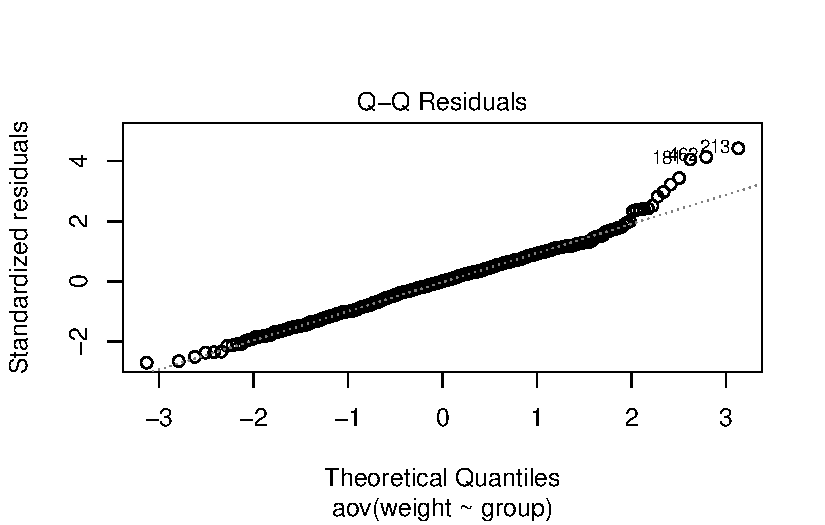
\includegraphics{ANOVA_files/figure-pdf/unnamed-chunk-14-1.pdf}

}

\end{figure}

Como todos los puntos caen aproximadamente a lo largo de esta línea de
referencia, podemos asumir la normalidad.

La conclusión anterior está respaldada por la \textbf{prueba de
Shapiro-Wilk} en los residuos ANOVA (W = 0.98151, p = 1.292e-06

) que no encuentra indicios de que se viole la normalidad.

\begin{Shaded}
\begin{Highlighting}[]
\CommentTok{\# Extract the residuals}
\NormalTok{aov\_residuals }\OtherTok{\textless{}{-}} \FunctionTok{residuals}\NormalTok{(}\AttributeTok{object =}\NormalTok{ res.aov )}
\CommentTok{\# Run Shapiro{-}Wilk test}
\FunctionTok{shapiro.test}\NormalTok{(}\AttributeTok{x =}\NormalTok{ aov\_residuals )}
\end{Highlighting}
\end{Shaded}

\begin{verbatim}

    Shapiro-Wilk normality test

data:  aov_residuals
W = 0.98151, p-value = 1.292e-06
\end{verbatim}

Tenga en cuenta que, una alternativa no paramétrica al ANOVA
unidireccional es la \textbf{prueba de suma de rangos} de
\textbf{Kruskal-Wallis}, que se puede usar cuando no se cumplen los
supuestos de ANNOVA.

\begin{Shaded}
\begin{Highlighting}[]
\FunctionTok{kruskal.test}\NormalTok{(weight }\SpecialCharTok{\textasciitilde{}}\NormalTok{ group, }\AttributeTok{data =}\NormalTok{ my\_data)}
\end{Highlighting}
\end{Shaded}

\begin{verbatim}

    Kruskal-Wallis rank sum test

data:  weight by group
Kruskal-Wallis chi-squared = 305, df = 1, p-value < 2.2e-16
\end{verbatim}



\end{document}
